The Electronic Marking System (EMS) allows students, teachers, headmasters and guardians to access students' marks of their units.  Each user is able to benefit from the system according to the powers/authorizations given to him/her.  For example, students can electronically submit papers (reports) for a particular unit to be marked by the unit's teacher.  Teachers, on the other hand, have the right to establish, edit and delete marks of their students.  In addition, headmasters and guardians can also access the system for the purpose of viewing marks and signing final reports.  

\begin{figure}[bht]
\centering
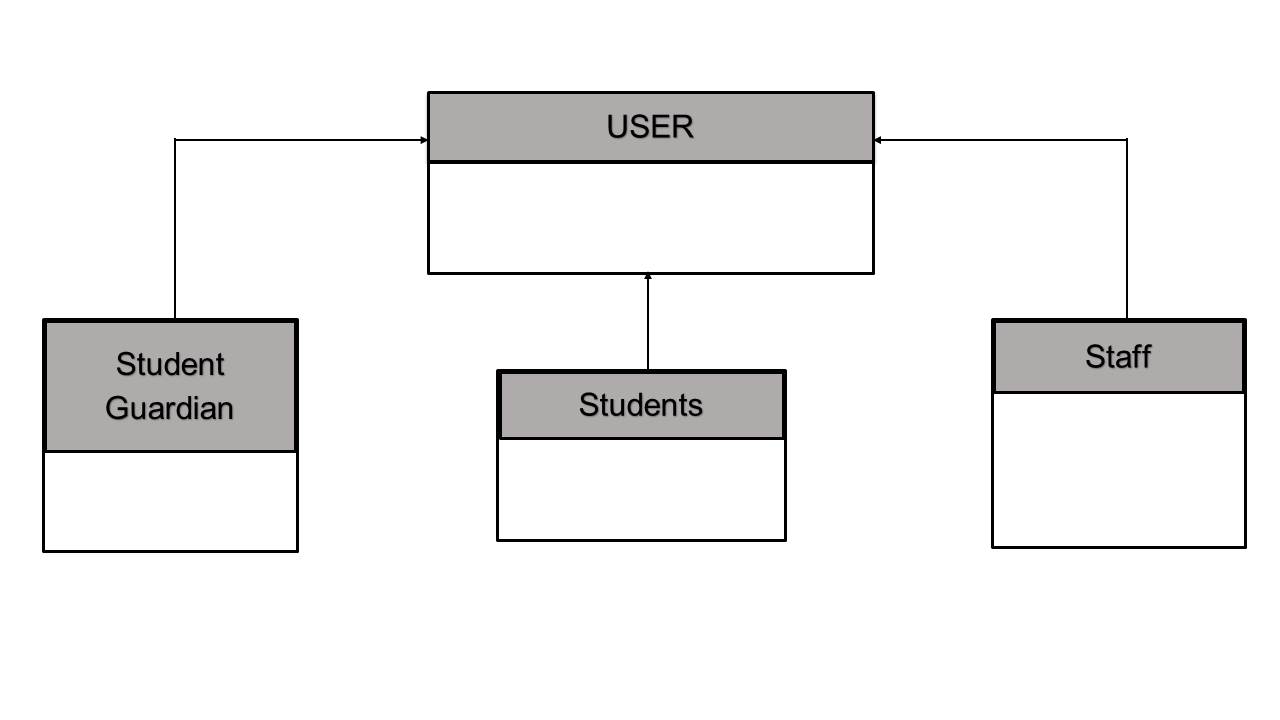
\includegraphics[scale=0.26]{EMSEntities.png}
\caption{Entities of the EMS's users.}
\label{fig:RBACPol}
\end{figure}

Generally, the EMS system can be accessed by different users: the system admin (who controls and manages the different entities and resources of the system), students, teachers, headmasters and guardians.  Hence, users can be classified into three main entities (tables): staff, students, and guardians, where staff entity represents teachers and headmasters as well as the system admin.
The other entities of the system as well as the relationships between those are briefly demonstrated in table \ref{tab:otherentities} and table \ref{tab:relations},respectively, in the following page.

\begin{table*}[bth]
\centering
\caption{Entities of the EMS System.}
\small
\rowcolors{0}{}{lightblue}
\begin{tabular}{p{0.8 in} p{6 in}} \hline 
\hline
Code & Description\\\hline\hline

UNIT& to represent all units taught at secondary schools. \\ 
SUBMISSION& to store submitted reports by students. \\ 
FINAL\_REPORT& contains final reports for all students. \\ 
MARK& its contents are natural numbers, which represent students' marks. \\ 
ROLES& this entity is set up for the purpose of applying RBAC model.  Hence, it represents the different roles in the EMS system (i.e. admin, teacher, student, etc.).\\ \hline\hline
\end{tabular}
\label{tab:otherentities}
\end{table*}




\begin{table*}[bth]
\centering
\caption{Relations between the EMS entities.}
\small
\rowcolors{0}{}{lightblue}
\begin{tabular}{p{0.9 in} p{5.9 in}} \hline 
\hline
Code & Description\\\hline\hline

studies &   a relation between a student and a unit; where each student studies more than one unit; and that unit can be registered for many students. \\

taughtBy &  a relation between a unit and a teacher; where each unit must be taught by at least one teacher; and that teacher can be registered to more than one unit.\\

hisGuardian &  a relation between a student and a guardian.  A student can have more than one guardian in order to facilitate the process of following up the student's level.  In addition, the guardian can be registered for more than one student\\

submits &   a relation between a student and a submission; where any student can submit any number of reports (depending on the unit and the academic level that a student is studying at).\\

reportFor &  a relation between a submitted report and a unit.  Therefore, all submitted reports are for particular units, and each unit may have more than one report. \\

submissionMark &  a relation between a submitted report and a mark (which is a natural number).  However, it is not possible for a report to be mapped into two different marks (axiomatic!), but we can find that a given mark represents the grade of more than one report.\\

InClassMark &  a relation between a unit and a mark (i.e. natural number) to specify a student's mark for his/her participations and activities inside the class during the year. \\

examMark &  a relation between a unit and a mark to specify the student's mark/s (depending on the number of exams for that unit).\\ 

studentReport &  a relation between a student and a final report; where each student must have a final report for each unit, which shows his/her final mark.  However, it is not reasonable to assign two final reports to the same student.\\

hasTheRole & maps a user into a set of roles (e.g. student, teacher, headmaster or student's guardian); where each user would be linked to only one role (unless there were some circumstances made otherwise, e.g. in case of absence of the school manager, any teacher can be assigned to play the role of headmaster; and this assignment falls under the responsibility of the system’s admin).

\\ \hline\hline
\end{tabular}
\label{tab:relations}
\end{table*}








